\chapter{Evaluierung}\label{kap:eval}

Dieses Kapitel beschreibt die Auswertung der
Ergebnisse der trainierten Modelle.

Dafür werden im ersten Abschnitt zunächst die Metriken 
erklärt, anhand denen die Evaluierung erfolgte. 

Im zweiten Abschnitt werden die beiden verwendeten Model
Architekturen SSD und Fater R-CNN hinsichtlich dieser Metriken, sowie anhand 
inferenzergebnisse verglichen.

Der dritte Abschnitt beschreibt Methoden mit denen 
die Ergebnisse das Faster R-CNN optimiert werden konnten und im 
vierten Abschnitt werden die Modelle noch einmal miteinander
verglichen, dieses mal hinsichtlich der Inferenzzeit.

\section{Evaluierungs Metriken}\label{sec:metricen}

\subsection*{Mean Average Precision (mAP)}

Zur Messung der Genauigkeit der Object Detection Modelle 
wurde die \textit{Mean Average Precision (mAP)} herangezogen.

Diese bezieht sowohl Klassifizierungs- als auch Lokalisierungsgenauigkeit 
mit ein und lässt sich den Folgenden Werten errechnen.

\begin{itemize}
  \item \textit{True Positive (TP)}: Das Model hat richtig das Vorhandensein eines Objekts geschätzt
  \item \textit{True Negative (TN)}: Das Model hat richtig die Abwesenheit eines Objekts geschätzt
  \item \textit{False Positive (FP)}: Das Model hat fälschlicherweise das Vorhandensein eines Objekts geschätzt
  \item \textit{False Negative (FN)}: Das Model hat fälschlicherweise die Abwesenheit eines Objekts geschätzt
\end{itemize}

Die festlegung, für True Positive Werte wird dabei über die 
Intersection over Union ermittelt.

Diese ist durch den Überlappungsgrad der gelabelten (Ground Truth) und der
geschätzete Boundig Box zu dem Gesammtbereich 
beider Boxen definiert.

Beträgt dieser mehr als ein bestimmter Threshhold, häufig 50\%,
gilt die Schätzung als \textit{True Positive}, andernfalls als 
\textit{False Positive}. 


\newcommand\MyBox[2]{
  \fbox{\lower0.75cm
    \vbox to 1.7cm{\vfil
      \hbox to 1.7cm{\hfil\parbox{1.4cm}{#1\\#2}\hfil}
      \vfil}%
  }%
}
\noindent
\renewcommand\arraystretch{1.5}
\setlength\tabcolsep{0pt}

\begin{minipage}{\textwidth}
    \begin{minipage}[b]{0.49\textwidth}
      \centering
      \def\svgwidth{0.8\textwidth}
      \input{Bilder/IoU_formula.pdf_tex}
      \captionof{figure}{Intersection over Union}
      \label{fig:iou}
  \end{minipage}
    \hfill
    \begin{minipage}[b]{0.49\textwidth}
      \centering
      \begin{tabular}{c >{\bfseries}r @{\hspace{0.7em}}c @{\hspace{0.4em}}c @{\hspace{0.7em}}l}
        \multirow{10}{*}{\rotatebox{90}{\parbox{2.5cm}{\bfseries\centering Tatsächlicher Wert}}} & 
          & \multicolumn{2}{c}{\bfseries Geschätzter Wert} & \\
        & & \bfseries p & \bfseries n & \bfseries\\
        & p$'$ & \MyBox{True}{Positive} & \MyBox{False}{Negative}\\[2.4em]
        & n$'$ & \MyBox{False}{Positive} & \MyBox{True}{Negative} \\
      \end{tabular}
        \captionof{figure}{Confusion Matrix}
    \end{minipage}
\end{minipage}

\vspace{1cm}

Anhand dieser, in der Confusion Matrix dargestellen, Werte 
lassen sich \textit{Precision} und \textit{Recall} berechnen.

Dabei ist der Recall definiert durch das Verhältniss der
richtig gefundenen zu allen im Bild befindlichen Objekten, 
oder anders ausgedrück die True Positives zu True Positive + 
False Negatives wie in Geichung \ref{eq:recall} dargestellt.

\begin{equation}
  \label{eq:recall}
  Recall = \frac{TP}{TP + FN}
\end{equation}

\vspace{0.5cm}

Im Gegensatz zu Recall welcher die Trefferquote angibt, 
gibt die Precision die Genauigkeit an mit der die Objekte
gefunden werden.

Die Precision ist durch das Verhältnis der Richtigen 
Schätzungen bezogen auf alle gemachten Schätzungen definiert, 
was durch die True Positives durch die True Positives + 
False Positives wie in Gleichung \ref{eq:precision}
dargestellt ausgedrückt wird.


\begin{equation}
  \label{eq:precision}
  Precision = \frac{TP}{TP + FP}
\end{equation}

\vspace{0.5cm}

Stellt man den Recall, welcher die Trefferquote angibt, und der 
Precision welche die genauiggkeit der treffer angibt gemeinsam 
dar ergibt sich die \textit{Precision-Recall-Kurve}, dessen 
Fläche die \textit{Average Prcision} für eine klasse darstellt.
Für alle Klassen im Mittel ergibt sich so die \textit{mean Average 
Precision}.

\vspace{0.5cm}

\begin{equation}
  Average Precision = \sum(Precision(Recall))
\end{equation}

\begin{equation}
  mAP = \frac{1}{N} \sum AP
\end{equation}

\vspace{0.5cm}





\subsection*{Fehlerfunktion (Loss)}
Die Fehlerfunktion setzet sich aus einem Lokalisierungs und einem 
Klassifizierungsfehler zusammen. 
Die Lokalisierung erfolgt über eine Lineare Regression zur 
Annäherung der Bounding Boxes and die richtigen Koordinaten.\\



%----------------- SECTION: validtaion ---------------------
\section{Vergleich der Modelle}\label{sec:model_vergleich}

Dieser Abschnitt beschreibt, wie die beiden für das Training 
verwendeten Object Detection Architekturen Single Shot Detector (SSD)
und Faster R-CNN mit verschiedenen 
CNNs und Datensatz aufbereitungen miteinander verglichen und 
ausgewertet wurden.


\subsection{Evaluierung/Validierung}

Folgen dargestellte Ergebnisse beziehen sich auf 
das Validierungsset des für das Training verwendeten 
OpenImages Datensatzes.

Die berechnung anhand der in \ref{sec:metricen} erläuterten 
Metriken konnte dabei mithilfe Tensorflow durchgeführt 
und schon während des Trainings mit in dem Evaluierungs-Tool 
Tensorboard visualisiert werden werden.

Bei den für das Training verwendeten Modellen handelt es sich zum einen 
um das SSD, für welches einmal das MobilenetV2 und einmals das InceptionV2
als Basis CNN verwendet wurden und zum anderen um das Faster R-CNN mit 
InceptionV2 als Basis CNN.


Diese wurden jeweils sowohl auf den augmentierten als auch auf 
den origanalen Datensatz trainiert. Eine Gegenüberstellung der 
Ergebnisse ist in Tabelle \ref{table:model_vgl} dargestellt.


% Tabelle \ref{table:model_vgl} zeigt die Trainingsergebnisse 
% der Loss und mAP Werte der Trainierten Modelle, welche aus SSD mit
% einmal MobilenetV2 und einmal InceptionV2 als Basis CNN sowie 
% Faster R-CNN nur mit InceptionV2 Ergebnisse 


% SSD wurd mit Batchsize=12 75k durchläufe trainiert.\\
% Faster R-CNN mit Batchsize=1 für 200k durchläufe.(1 weil dynamische input size)\\
% eine epoche sind (teps mal batchsize)/samples
\vspace{0.5cm}
\begin{table}[H]
  \label{table:model_vgl}
  \centering
  \begin{tabular}{m{0.25\textwidth}m{0.2\textwidth}|m{0.15\textwidth}<{\centering}m{0.15\textwidth}<{\centering}}
  \hline
  Model                                                              & Optimierung                                                                   & mAP                                                        & Loss                                                       \\ \hline\hline
  SSD + MobilenetV2                                                  & \begin{tabular}[c]{@{}l@{}}Ohne\\ Augmentierung\end{tabular}                  & \begin{tabular}[c]{@{}l@{}}0,62\\ 0,61\end{tabular}        & \begin{tabular}[c]{@{}l@{}}3,56\\ 3,50\end{tabular}        \\ \hline
  SSD + InceptionV2                                                  & \begin{tabular}[c]{@{}l@{}}Ohne\\ Augmentierung\end{tabular}                  & \begin{tabular}[c]{@{}l@{}}0,65\\ 0,62\end{tabular}        & \begin{tabular}[c]{@{}l@{}}3,86\\ 3,71\end{tabular}        \\ \hline
  \begin{tabular}[c]{@{}l@{}}Faster R-CNN\\ +InceptionV2\end{tabular} & \begin{tabular}[c]{@{}l@{}}Ohne\\ Augmentierung\\ Early Stopping\end{tabular} & \begin{tabular}[c]{@{}l@{}}0,67\\ 0,69\\ 0,67\end{tabular} & \begin{tabular}[c]{@{}l@{}}0,82\\ 0,67\\ 0,69\end{tabular} \\ \hline
  \end{tabular}
\end{table}
\vspace{0.5cm}

All Modell weisen eine Verbesserung des Loss Wertes durch 
Augmentierung der Daten auf.
Bei den Konfigurationen mit SSD führte die Augmentierung jedoch auch 
zu einer verringerung des mAPs, was auf die geringere Komplexität 
und damit weniger Möglichkeiten sich an die Augmentierten Daten 
Anzupassen zurückzuführen ist.
Die höhere Komplexeität des Fster R-CNN bring auf der 
anderen Seite auch eine höhere Wahrscheinlich keit zum 
Ovefitting mit.

 
Daher ist hier die Auswirkung der Augmentierung am 
effekitvsten, was anhand der Trainingsverläufer 
der mAP und Loss kurven dargestellt in Abb 
\ref{plot:mAP} und \ref{plot:loss} zu 
erkennen ist.

Die Loss Kurve nimmt bei den nicht augmentierten Datensatz ab 
ca 100000 Schritten wieder zu, was ein hinweis dafür ist, 
das Overfitting stattgefunden hat.

Durch die Augmentierung der Daten konnte der Loss Wert 
auf dem erreichten Niveau gehalten werden.

Als weitere Strategie zur vermeiden von Overfittung wurde 
hier auch Early Stopping angewendet, dabei wird das Training
bevor der Loss Wert anfängt wieder anzusteigen unterbrochen.

Anhand der Losskurven kann man erkennen das sich dadurch 
die gleichen Werte wie durch Augmentierung erreichen lassen.

Jedoch zeigt sich auch anhand der mAP Kurve, dass 
durch das frühzeitige Stoppen der mAP Wert nicht die 
Chnace hat seinen Endwert zu erreichen und somit 
unterhalb des mAP Werts bei Augmentierten Daten bleibt.


\vspace{0.5cm}

\begin{figure}[H]
\begin{minipage}{0.5\textwidth}
  \centering
  \label{plot:mAP}
  \def\svgwidth{0.9\textwidth}
  \input{Bilder/plots/overfitting_kein_early_aug_mAP.pdf_tex}
  \captionof{figure}{mAP}
\end{minipage}
\begin{minipage}{0.5\textwidth}
  \centering
  \label{plot:Loss}
  \def\svgwidth{0.9\textwidth}
  \input{Bilder/plots/overfitting_kein_early_aug_loss.pdf_tex}
  \captionof{figure}{Loss}
\end{minipage}
\end{figure}

% Legende: Overfitting
\begin{table}[htb]
  \centering
  \begin{tabular}{m{0.1\textwidth}<{\centering}m{0.2\textwidth}<{\centering}m{0.2\textwidth}<{\centering}}
    $\color[HTML]{FF7043}\medbullet$  Ohne & $\color[HTML]{0077BB}\medbullet$  Early Stopping & $\color[HTML]{CC3311}\medbullet$  Augmentierung
  \end{tabular}    
\end{table}

% colors
% orange: FF7043
% blue  : 0077BB
% red   : CC3311


%----------------- SECTION: Test Inferenz ---------------------
\subsection{Test Inferenz}\label{sec:test_inferenz}

Um eine bessere Vorstellung davon zu bekommen wie sich die 
unterschiedlichen Ergebnisse in mAP und Loss in der Anwendung 
tatsächlich bemerkbar machen, wurde die Inferenz der drei modelle 
für verschiedene Test Bilder durchgeführt.

Dafür wurden die Modelle in die für OpenVino benötigte Intermediate
Representation umgewandelt um dann mihilfe eines Python 
Scripts in die InferenceEngine geladen zu werden.

Mithilfe dieses Scripts konnten nun die Inferenz für 
folgende Testszenarien:

\begin{itemize}
  \item inferenz auf Test Set \textit{OpeImages}
  \item inferenz auf \textit{The iWildCam 2019 Dataset}\cite{beery2019iwildcam}
  \item inferenz auf eigene Bilder
\end{itemize}


\subsubsection{Test Set (OpenImages)}
Sowohl SSD als auch Faster R-CNN erkennen das meiste, da gr 
ähnlichkeit zu Trainingssatz.

Wenn jedoch mehrere Tiere im Bild sind, diese weiter weg oder schlechtere
Bildqualität, erkennt Faster R-CNN besser. Abb \ref{fig:faster_rcnn}
\\[1cm]
\begin{minipage}{0.5\textwidth}
  \centering
  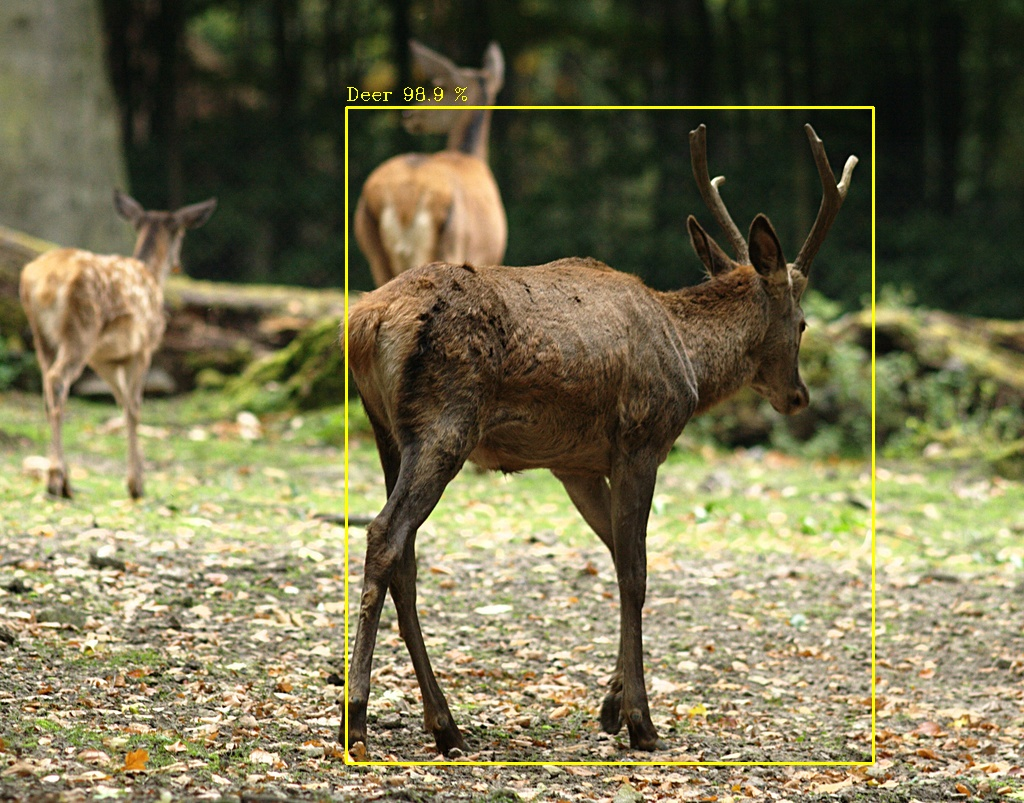
\includegraphics[width=0.9\textwidth]{model_compare_test__ssd_inception_v2.jpg}
  \captionof{figure}{SSD}
  \label{fig:ssd}
\end{minipage}
\begin{minipage}{0.5\textwidth}
  \centering
  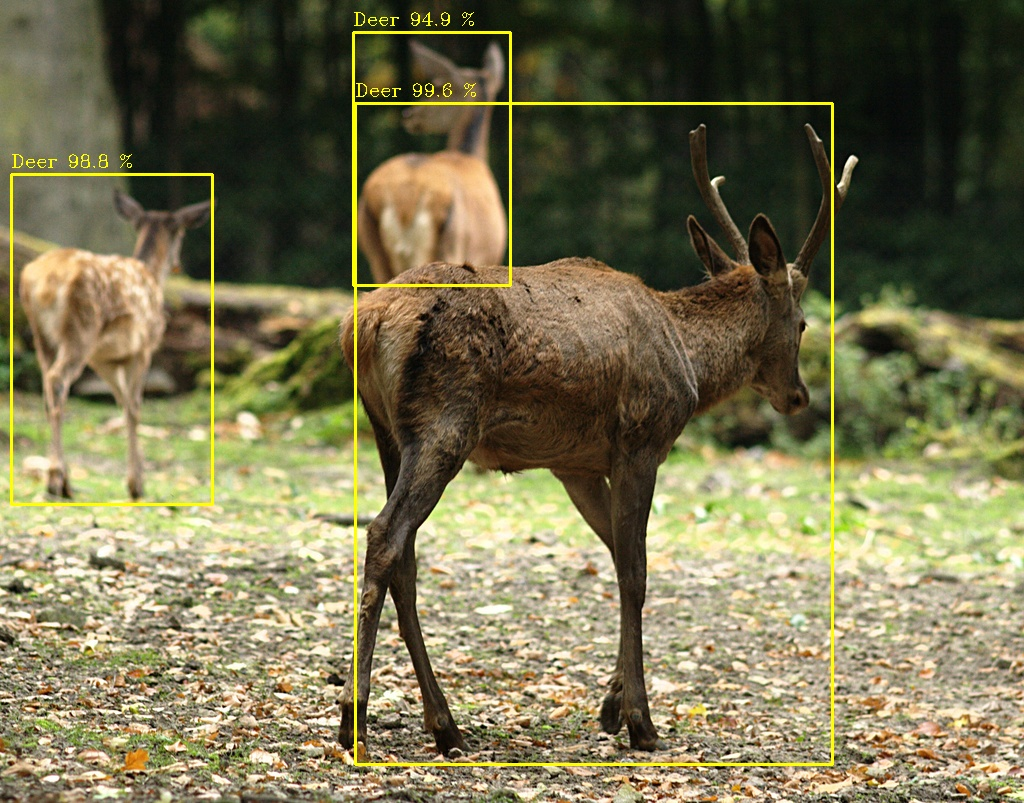
\includegraphics[width=0.9\textwidth]{model_compare_test__faster_rcnn_inception_v2_early_stopping.jpg}
  \captionof{figure}{Faster R-CNN}
  \label{fig:faster_rcnn}
\end{minipage}


\subsubsection{Eigene Aufnahmen}

\begin{minipage}{0.5\textwidth}
  \centering
  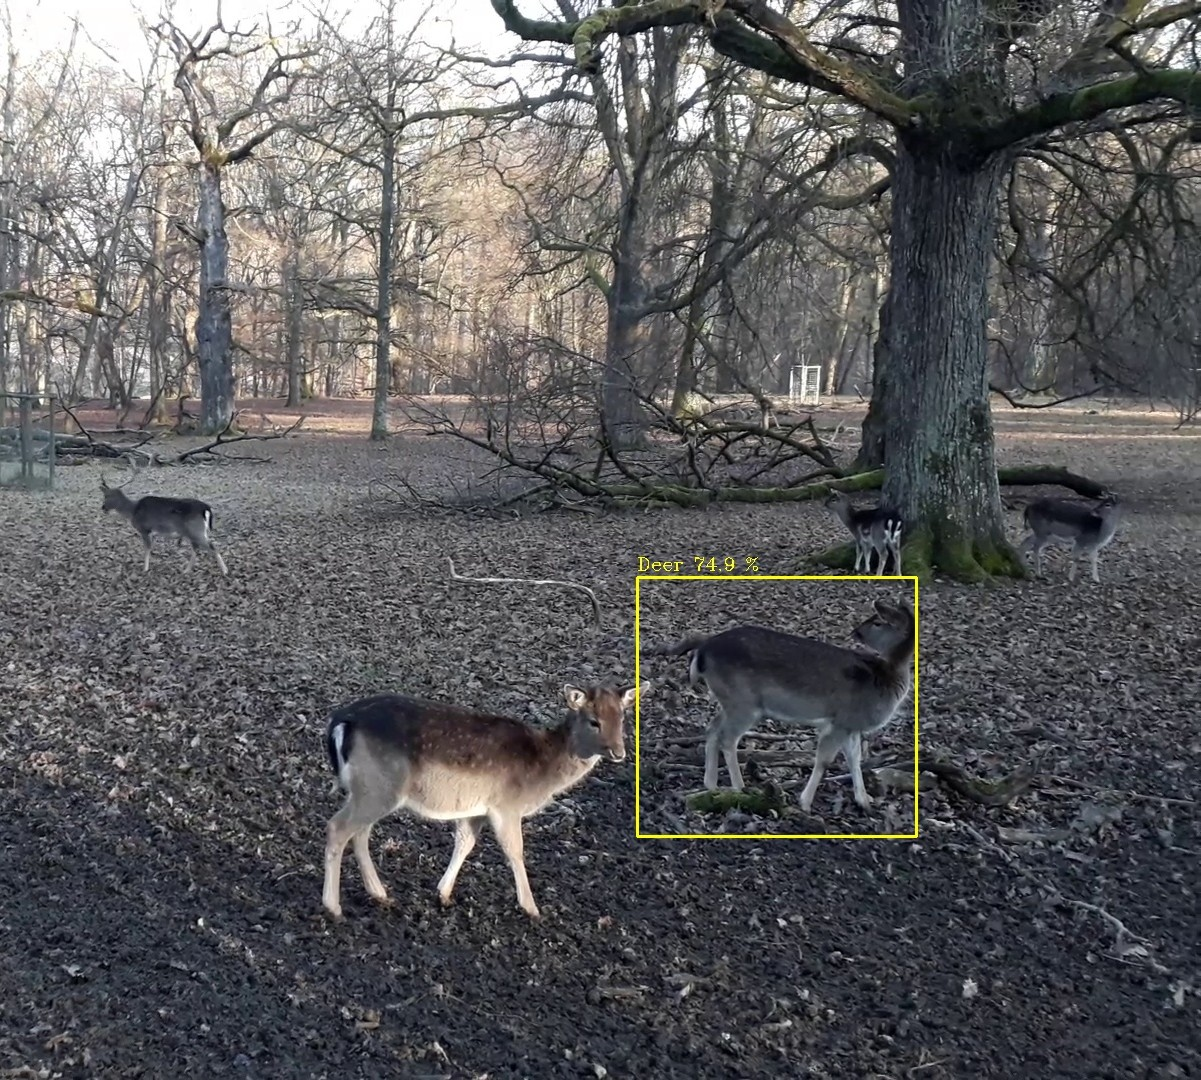
\includegraphics[width=0.9\textwidth]{model_compare_handy_ssd_mobilenet_v2.jpg}
  \captionof{figure}{SSD Mobilnet}
  \label{}
\end{minipage}
\begin{minipage}{0.5\textwidth}
  \centering
  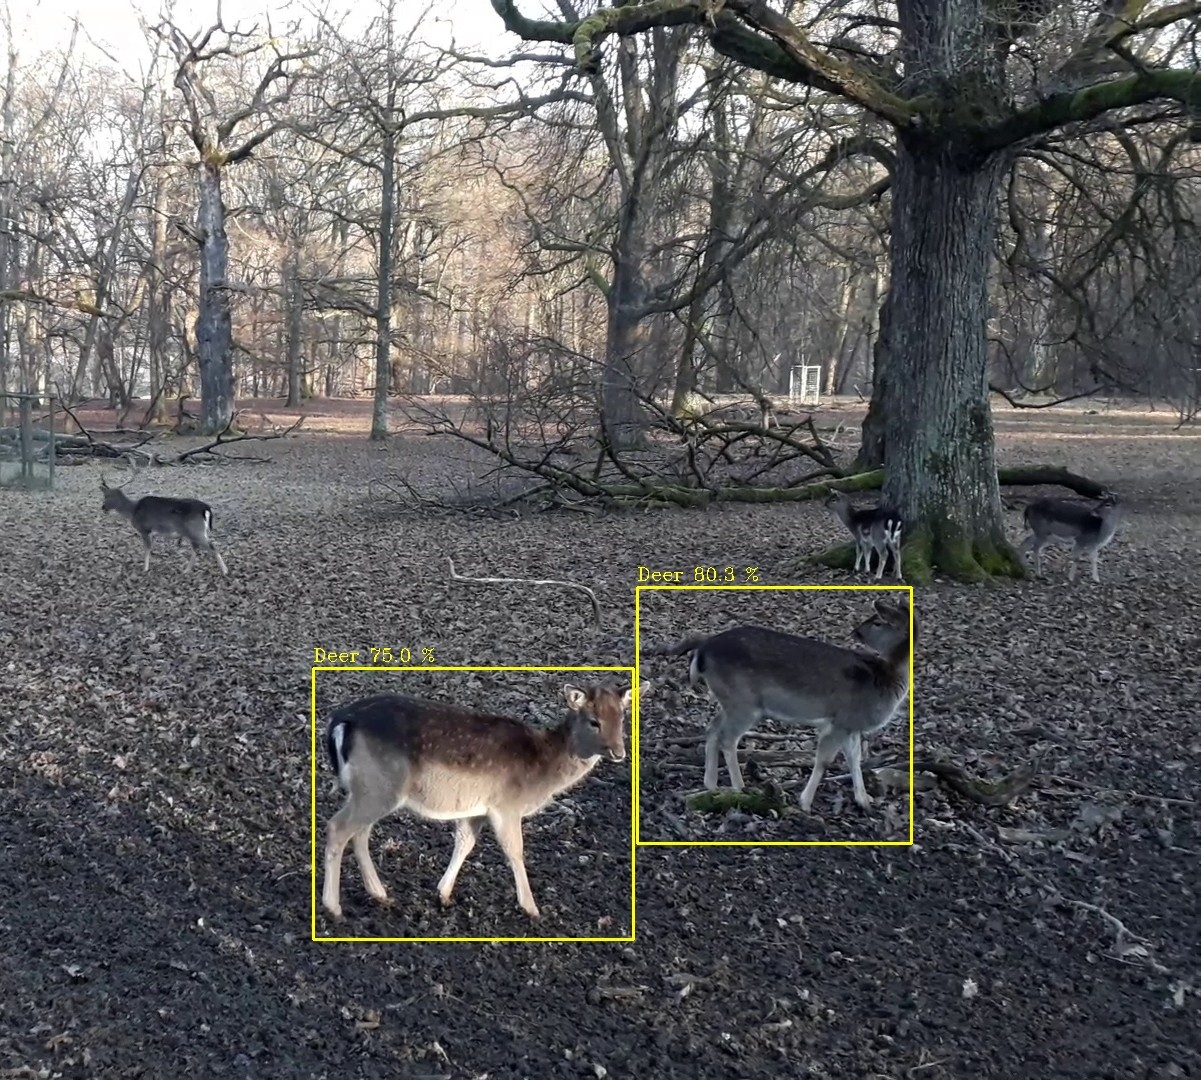
\includegraphics[width=0.9\textwidth]{model_compare_handy_ssd_inception_v2.jpg}
  \captionof{figure}{SSD Inception}
  \label{}
\end{minipage}
\\[1cm]
\begin{minipage}{0.5\textwidth}
  \centering
  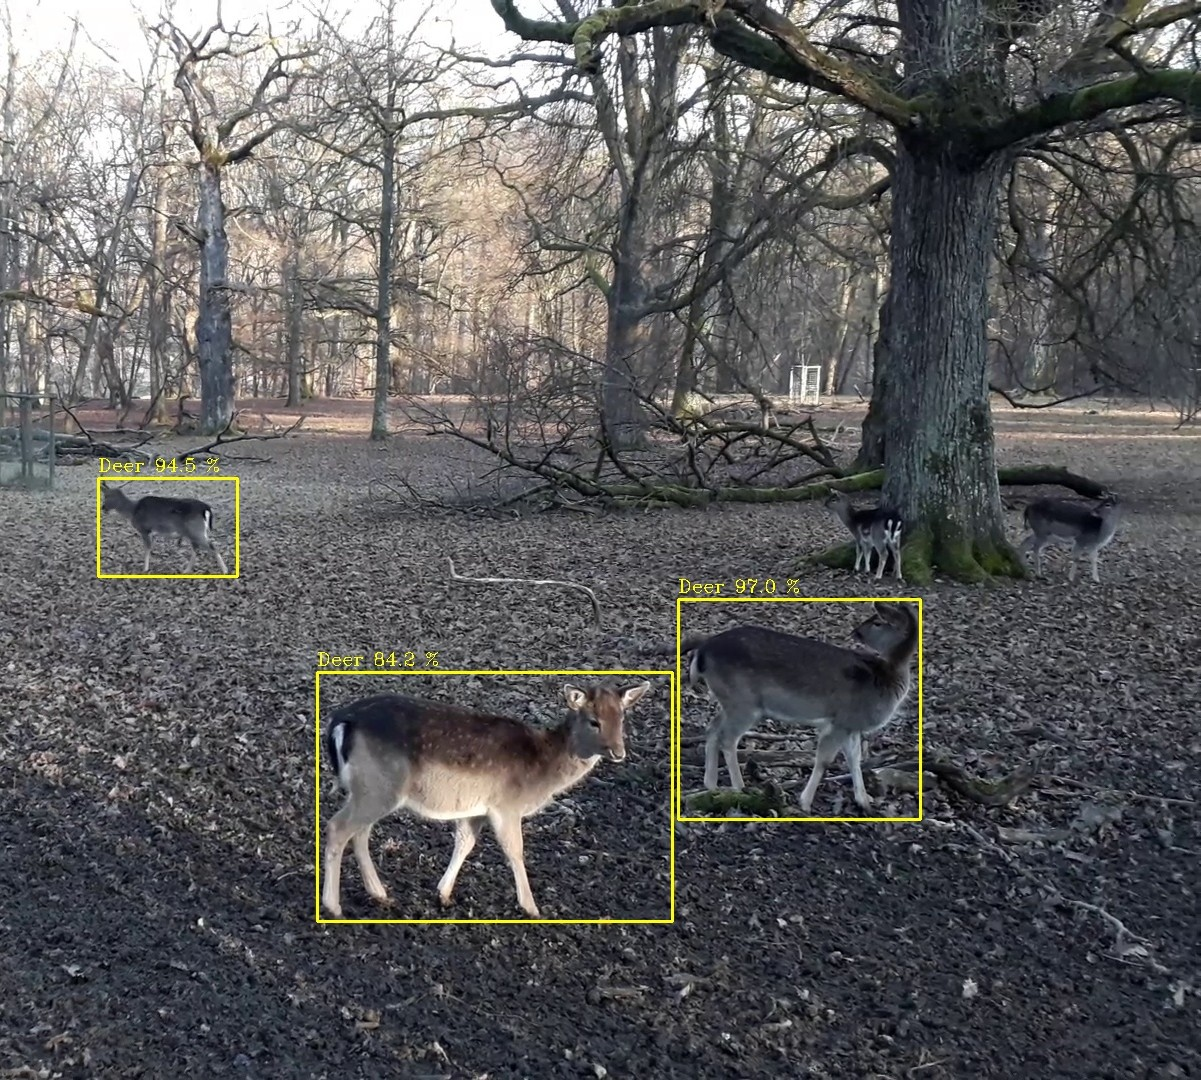
\includegraphics[width=0.9\textwidth]{model_compare_handy_faster_rcnn_inception_v2_early_stopping_ohne_aug.jpg}
  \captionof{figure}{Faster R-CNN + Early Stopping}
  \label{}
\end{minipage}
\begin{minipage}{0.5\textwidth}
  \centering
  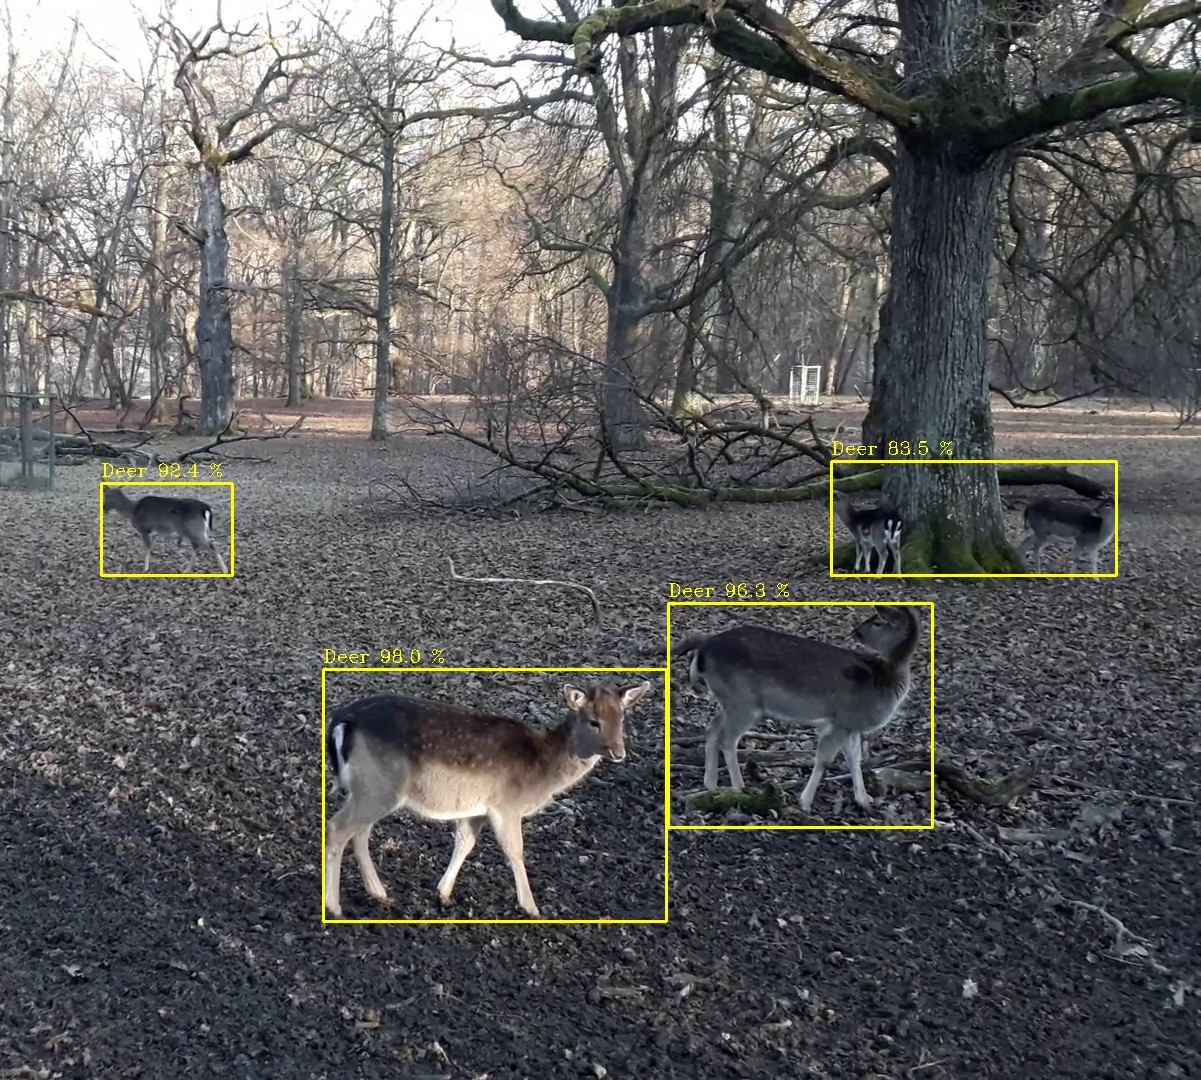
\includegraphics[width=0.9\textwidth]{model_compare_handy_faster_rcnn_inception_v2_early_stopping.jpg}
  \captionof{figure}{Faster R-CNN + Aug}
  \label{}
\end{minipage}


\subsubsection{iWildCam}

Aufnahmen von ... enthällt viele schlecht beleuchtete nacht Aufnahmen 
mit Infrarot Kamera, also ähnlich dem gewünschten Anwendungsfall.
Auch hier erkennt das Faster R-CNN am beste, jedoch 
schneiden hier alle schlecht ab.

Daher wurde, wie im nächsten Abschnitt beschrieben, versuch
das Faster R-CNN noch weiter zu optimieren.


%----------------- SECTION: optimierung ---------------------
\section{Optimierungen: Faster R-CNN}\label{sec:optimierung_faster_rcnn}


Als Ausgangslage zur verbesserung der Ergebnisse diente 
nun das Faster R-CNN mit augmentiertem Datensatz, welches 
im vorherigen Abschnitt die besten Resultate erzielte.

Auch hier werden zunächst die Ergebnisse zunächst wieder 
anhand der Eval Metriken für den Validierungsdatensatz mithilfe Tensorboard 
dargestellt und anschließend mit Testdatensatz sowie weitere testinferez 
durchgeführt.




\subsection{Verschiedene Augmentierungen}

Der erste Anstz war es dieses mit variierendem Augmentierungsgrad 
für insgesamt mehr Trainingsdurchläufe (500 statt 200) zu 
trainieren.

Im vorherigen Abschnitt wurde für die Augmentierung der 
Daten je Bild zufällig aus einer auswahl eine geometrische und eine 
Pixelbezogene augmentierungstechnik angewendet, sodass für jede Klass 
3000 Samples genriert wurden.

Als vairation wurde hier nun einmal die gleiche Augmentierungsstrategie 
für 4000 samples und einmal nur einer Augmentierung pro Bild für 
3000 Samples angewendet.

Die Trainingskurven aus Tensorboard sind für mAP und Loss sind in den
Plots \ref{plot:map_diff_aug} und \ref{plot:loss_diff_aug} dargestellt.
\vspace{1cm}

\begin{minipage}{0.5\textwidth}
  \centering
  \label{plot:map_diff_aug}
  \def\svgwidth{0.9\textwidth}
  \input{Bilder/plots/diff_aug_map.pdf_tex}
  \captionof{figure}{mAP}
\end{minipage}
\begin{minipage}{0.5\textwidth}
  \centering
  \label{plot:loss_diff_aug}
  \def\svgwidth{0.9\textwidth}
  \input{Bilder/plots/diff_aug_loss.pdf_tex}
  \captionof{figure}{Loss}
\end{minipage}

% Legende
\begin{table}[htb]
  \centering
  \begin{tabular}{m{0.1\textwidth}<{\centering}m{0.2\textwidth}<{\centering}m{0.2\textwidth}<{\centering}}
    $\color[HTML]{CC3311}\medbullet$  1 je bild & $\color[HTML]{FF7043}\medbullet$  3000 samples & $\color[HTML]{0077BB}\medbullet$  4000 samples
  \end{tabular}    
\end{table}

Es ist zu erkennen, das sich durch stärkere augmentierung der Trainingsdaten
der Loss reduzieren lässt, dadurch jedoch auch der mAP abnimmt.

% colors
% orange: FF7043
% blue  : 0077BB
% red   : CC3311



\subsection{weitere Regularisierungen}

Um das trotz Augmentierung zu stande kommende Overfitting zu 
vermeiden, wurden nun zusätzlich die L2 Regularisierung angewendet.
Diese soll wie in den Grundlagen (\ref{subsec:validation}) beschrieben, 
durch anfügen der aufsummierten Geweichte an die Loss Funktion, 
die Überanpassugne eindämmen.

In der Konfigurationsdatei des Fater R-CNN kann dies durch setzten des 
bestimmten Parameters für sowohl die erste Stufe, das RPN (Region Proposal Network)
als auch für die 2. Stufe, das Klassifizierungsnetz seperat gesetz werden.


Ebenso lassen sich die beiden Losskurven, aus denen sich der gesammt 
Loss zusammensetz, seperat anzeigen, wie in Plot \ref{plot:aug_l2_classifier_loss}
und \ref{plot:aug_l2_rpn_loss} zu erkennen ist.

Dadurch ließ sich feststellen, dass Overfitting nur beim Loss des RPNs 
stattfindet, weshalb der L2 Parameter auch nur für die erste Stufe 
das RPN engestellt wurde. Dabei wurde der Fa $\lambda = 0.001$ verwendet.

Schaut man nun wieder die beiden Losskurven an, zeigt sich deutlich der 
Effekt, den die L2 Regularisierung auf den RPN Loss hat, was sich dann 
auch im Gesammtloss durch eine leichte verbesserung bemerkbar machte.

\vspace{1cm}


\begin{minipage}{0.5\textwidth}
  \centering
  \def\svgwidth{0.9\textwidth}
  \input{Bilder/plots/aug_l2_mAP.pdf_tex}
  \captionof{figure}{mAP}
  \label{plot:aug_l2_mAP}
\end{minipage}
\begin{minipage}{0.5\textwidth}
  \centering
  \def\svgwidth{0.9\textwidth}
  \input{Bilder/plots/aug_l2_total_loss.pdf_tex}
  \captionof{figure}{Total Loss}
  \label{plot:aug_l2_total_loss}
\end{minipage}
\\[1cm]
\begin{minipage}{0.5\textwidth}
  \centering
  \def\svgwidth{0.9\textwidth}
  \input{Bilder/plots/aug_l2_classifier_loss.pdf_tex}
  \captionof{figure}{Classifier Loss}
  \label{plot:aug_l2_classifier_loss}
\end{minipage}
\begin{minipage}{0.5\textwidth}
  \centering
  \def\svgwidth{0.9\textwidth}
  \input{Bilder/plots/aug_l2_rpn_loss.pdf_tex}
  \captionof{figure}{RPN Loss}
  \label{plot:aug_l2_rpn_loss}
\end{minipage}
\begin{table}[htb]
  \centering
  \begin{tabular}{m{0.3\textwidth}<{\centering}m{0.4\textwidth}<{\centering}}
    $\color[HTML]{CC3311}\medbullet$  nur Augmentierung & $\color[HTML]{0077BB}\medbullet$  Augmentierung+L2 Regulierung
  \end{tabular}    
\end{table}

\vspace{1cm}

Dies wurde ebenso auf das Training mit weniger stark augmentiertem Datensatz
angewendet. Weitere Einstellungen waren $\lambda = 0.002$ und das 
ebenfalls in \ref{subsec:validation} beschriebene Dropout.
Die ergebnisse sind nocheinmal zusammefassend in Tabelle ... dargestellt.


\begin{table}[htb]
  \centering
  \label{table:reg}
  \begin{tabular}{m{0.2\textwidth}|m{0.2\textwidth}<{\centering}m{0.2\textwidth}<{\centering}m{0.2\textwidth}<{\centering}}
  \hline
  \textgreater 400k & mAP  & Loss (Gesammt) & Loss (RPN) \\ \hline\hline
  Augmentierung     & 0,7  & 0,74           &  0,12          \\
  +Dropout          & 0,7  & 0,73           &            \\
  +L2 Reg (0.01)    & 0,7  & 0,69           &            \\
  +L2 Reg (0.02)    & 0,69 & 0,7            &            \\ \hline
  \end{tabular}
  \caption{Regularisierungen}
\end{table}


\subsection{Test Inferenz}

Auch hier wurde nun wieder zur besseren Auswertung der Ergebnisse die 
Inferez Testweise auf die drei Datensätze Test Set des trainierten Open Images
Datensatzes, eigen Aufnahmen, sowie des \textit{iWildCam} Datensatzes durchgeführt.

\begin{minipage}{0.333\textwidth}
  \centering
  \label{}
  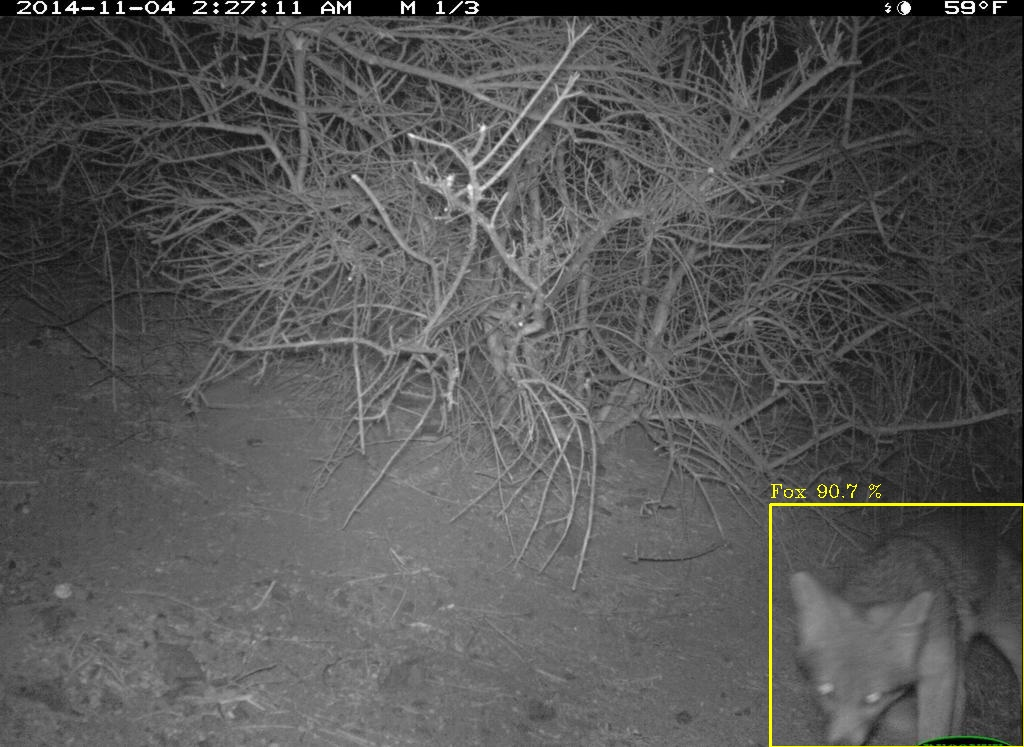
\includegraphics[width=\textwidth]{infer_images/iWildCam/fox/cut/59df5ee1-23d2-11e8-a6a3-ec086b02610b_faster_rcnn_inception_v2_3000.jpg}
  \captionof{figure}{3000 Samples}
\end{minipage}
\begin{minipage}{0.333\textwidth}
  \centering
  \label{}
  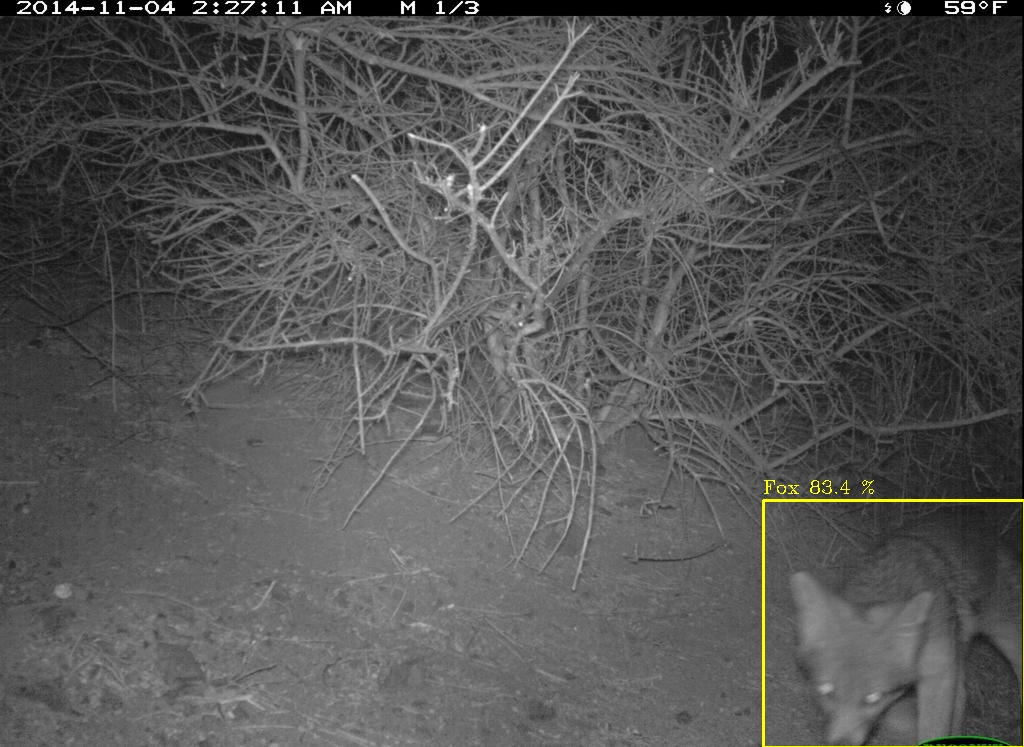
\includegraphics[width=\textwidth]{iWildCam/fox/cut/59df5ee1-23d2-11e8-a6a3-ec086b02610b_faster_rcnn_inception_v2_4000.jpg}
  \captionof{figure}{4000 Samples}
\end{minipage}
\begin{minipage}{0.333\textwidth}
  \centering
  \label{}
  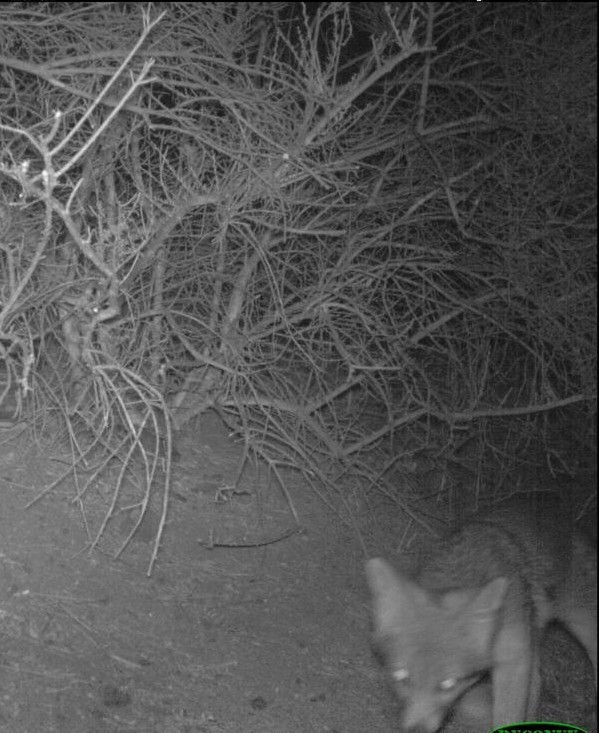
\includegraphics[width=\textwidth]{iWildCam/fox/cut/59df5ee1-23d2-11e8-a6a3-ec086b02610b_faster_rcnn_inception_v2_less_aug.jpg}
  \captionof{figure}{50\% Augment}
\end{minipage}

Bei der L2 Regulariesierung konnte für das iWildCam keine verbesserung festgestellt werden,
teilweise wurden die Bilder besser erkannt, teilweise schlechter, so dass im 
Mittel keine Verbesserung entstand.

Für die eigenen Bilder waren die Ergebnisse sogar schlechter.


\begin{minipage}{0.5\textwidth}
  \centering
  \label{}
  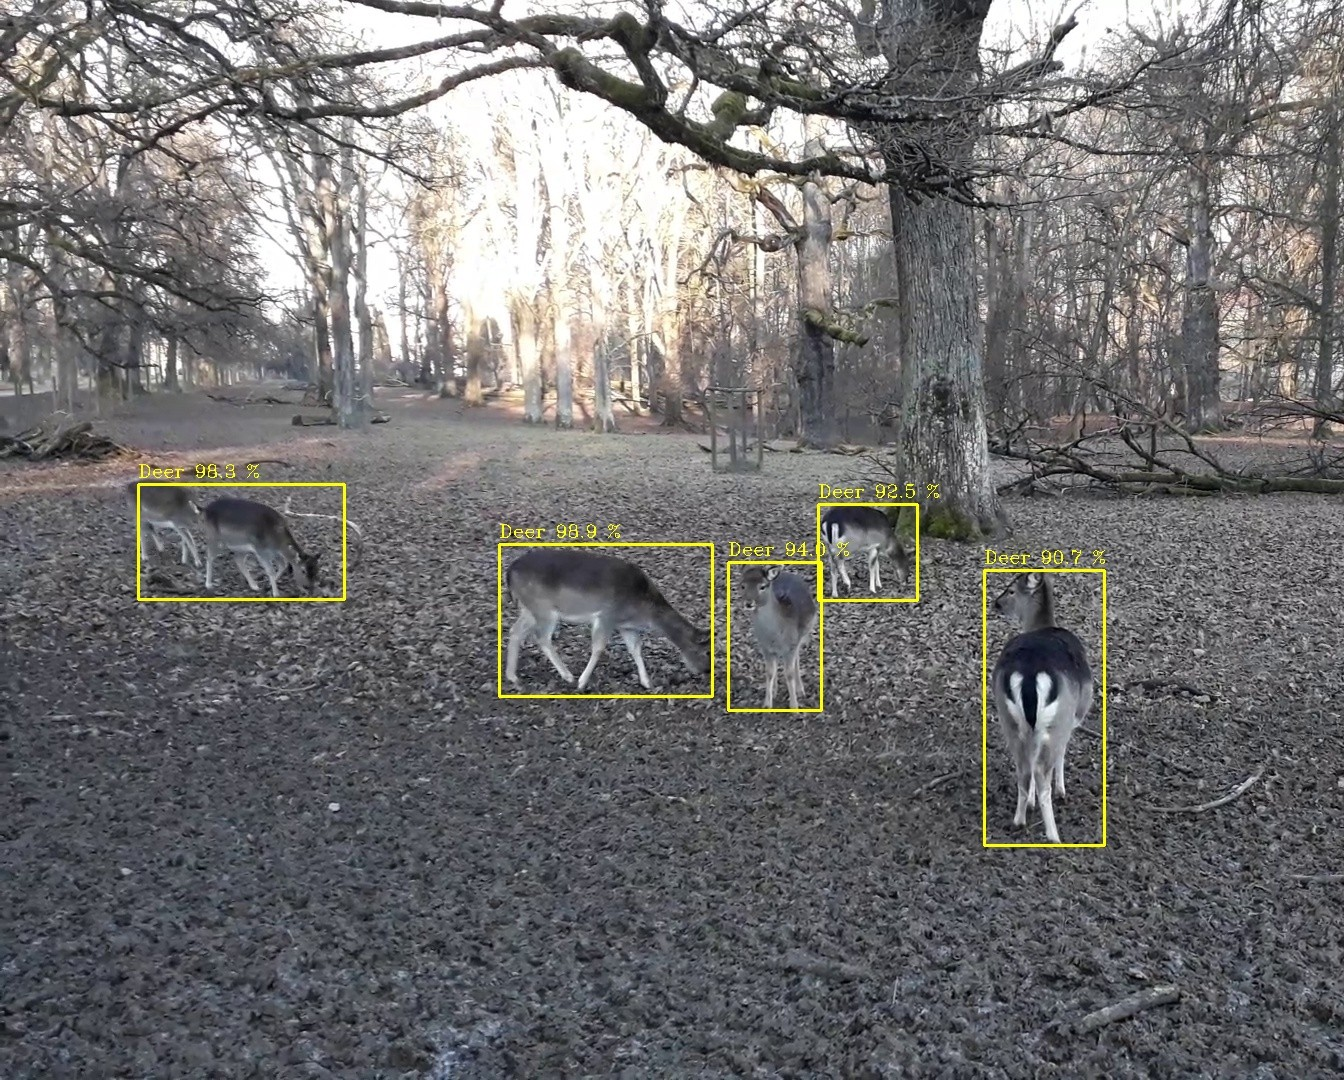
\includegraphics[width=0.95\textwidth]{eigene/20191229_145616_frame_20_faster_rcnn_inception_v2_3000.jpg}
  \captionof{figure}{}
\end{minipage}
\begin{minipage}{0.5\textwidth}
  \centering
  \label{}
  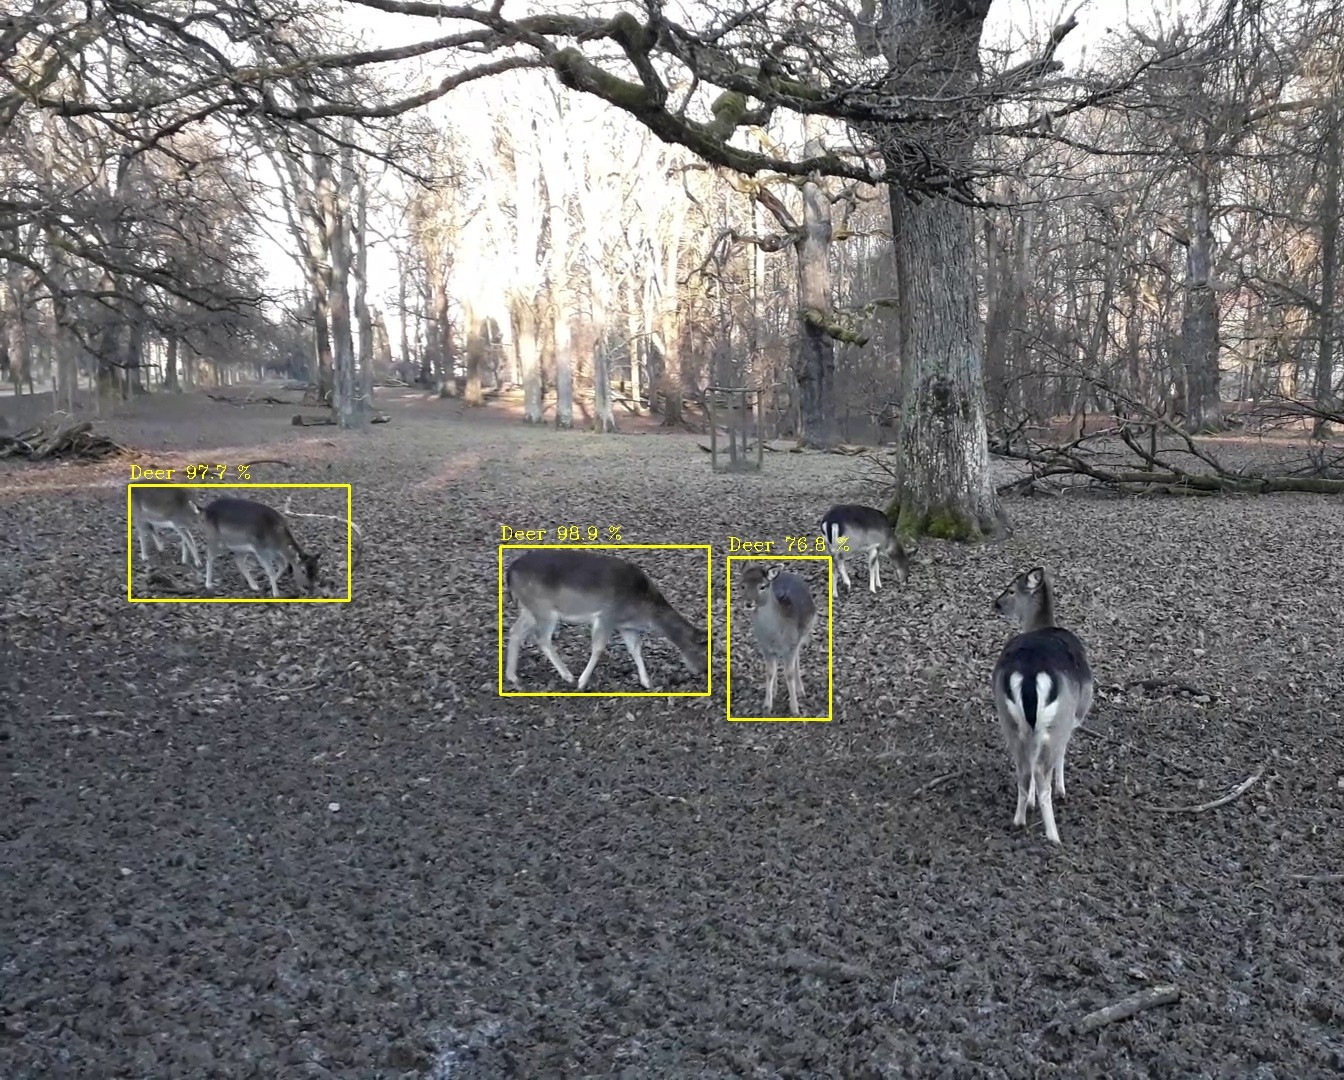
\includegraphics[width=0.95\textwidth]{eigene/20191229_145616_frame_20_faster_rcnn_inception_v2_l2.jpg}
  \captionof{figure}{}
\end{minipage}



Daraus lässt sich schließen das die Art/Qualität/Varianz der Daten 
den größeren einfluss auf das ergebniss haben und mit den Hyperparametern 
wenn überhaup



\subsection{Graustufen}
da kamerea graustufen bilder liefert, wurde getestet, ob ein 
training in graustufen bilder zu besseren erg führt, ... nicht so.



% \subsection{weitere tabellen}\label{subsec:regularisierung}

% \begin{table}[htb]
%     \centering
%     \label{tab:regularization}
%     \begin{tabular}{| l || c | c | c | c |} 
%         \hline
%         Regularisierung & $mAP_{orig}$ & $mAP_{handy}$ & $Loss_{orig}$ &  $Loss_{handy}$\\
%         \hline
%         Early Stopping (100k steps) & 0.6715 & 0.4265 & 0.6742 & 0.267\\
%         \hline
%         Augmentierung (200k steps) & 0.6914 & 0.4537 & 0.6738 & 0.2503\\ % hier noch verschiedene kombinationen von augmentierungen
%         \hline
%     \end{tabular}        
%     \caption{Regularization}
% \end{table}




% \subsection{Graustufen/Infrarot Bilder}\label{subsec:eval_gray}


% \begin{table}[htb]
%     \centering
%     \label{tab:eval_gray}
%     \begin{tabular}{| l | l || c | c |} 
%         \hline
%         Modell & Dataset & mAP & Loss\\
%         \hline
%         \multirow{2}{*}{rgb} & original & 0.6556 & 0.1451 \\
%         & handy & 0.4155 & 0.2389 \\
%         \hline
%         \multirow{2}{*}{gray 1 channel} & original & 0.5625 & 0.1716 \\
%         & handy & 0.3226 & 0.2747 \\
%         \hline
%         \multirow{2}{*}{gray 3 channel} & original & 0.664 & 0.1653 \\
%         & handy & 0.438 & 0.2492 \\
%         \hline
%     \end{tabular}        
%     \caption{Grayscale}
% \end{table}





\section{Inferenz zeit}\label{sec:infertime}

Neben der Genauigkeit ist die Ausführungszeit welche ein Model für die 
Inferenz benötigt, ein weiteres kriterium für die auswahl des Modells gewesen.
Je nach Anwendungsart muss diese in Echtzeit erfolgen oder nicht.

Ein Faktor von dem die Inferenzzeit abhängt ist die verwendeten Hardware
sowie Library. Für den Neural Compute Stick können dafür OpenCV oder 
OpenVino verwendetet werden, wobei mit OpenVino die möglichkeit 
zur asynchrone Inferenzausführung sowie mehreren Inferenz Requests wodurch 
sich die Inferenz zeit optimieren lässt.


Der zwiete Faktor wird durch die Komplexität des CNNs und der
zur Objekterkennung verwendeten Architektur bestimmt.

Üblicherweise sind Komplexere Modelle wie Faster R-CNN genauer jedoch 
auch langsamer.

Im folgenden soll daher zunächst die Asynchrone Inferenz näher 
erläutert werden und anschließen ein verfahren zur Untersuchung 
des Einfluss der Art der trainierten Modelle auf die Inferenz Zeit.

\subsection{Asychrone Inferenz}

Bei einem Synchronen inferenzablauf kann immer nur entweder inferiert oder 
die Daten vor- und nachverarbeitet werden. Da die inferenz jedoch auf dem 
Chip des NCS2 und nicht auf dem Pc oder Raspberry läuft, kann diese auch 
ungehindert parallel dazu ablaufen, was in OpenVino mit der Asychronen Api 
erreicht werden kann.

\vspace{1cm}
\begin{minipage}{0.1\textwidth}
  \hfill
\end{minipage}
\begin{minipage}{0.5\textwidth}
  \begin{algorithm}[H]
    \caption{Synchrone Inferenz}
    \begin{algorithmic}
    \WHILE{\TRUE}
        \STATE capture FRAME
        \STATE preprocess CURRENT InferRequest
        \STATE \textbf{start} CURRENT InferRequest
        \STATE \textbf{wait} for CURRENT InferRequest
        \STATE process CURRENT result
    \ENDWHILE
    \end{algorithmic}
  \end{algorithm}  
\end{minipage}
\begin{minipage}{0.4\textwidth}
  \centering
  \vspace{1cm}
  \def\svgwidth{0.5\textwidth}
  \input{Bilder/sy_asy_legend.pdf_tex}
\end{minipage}

\vspace{1cm}
\begin{figure}[H]
  \centering
  \def\svgwidth{0.8\textwidth}
  %\tikzset{
    desicion/.style={
        diamond,
        draw,
        text width=4em,
        text badly centered,
        inner sep=0pt
    },
    block/.style={
        rectangle,
        draw,
        text width=5em,
        text height=1em,
        text centered
    },
    arrow/.style={
        draw,
        >=latex,
        ->
    }
}


\begin{tikzpicture}

    \node(infer1) [block] {infer1};
    \draw[arrow] (0,-1em) -- (10,-1em);
    % \node (A) [desicion] {entschei\\dung};
    % \node (B) [block, below of=A, node distance=5cm, text width=5em] {bock};
    % \node (C) [block, right of=A, node distance=5cm] {noch ein\\bock};


    % \draw[arrow] (A) --  node [left, fill=white] {yes} (B);
    % \draw[arrow] (A) -- node [below, near end] {crap} (C); 
    % \draw[arrow] (B) -| node [near start, fill=white] {yes} (C);

\end{tikzpicture}

  \input{Bilder/sync_infer.pdf_tex}
  \caption{}
  \label{}
\end{figure}

djfoiadshilfh
\\
asdfpiuhasdog\\
söodfhas\\
aidfh


\vspace{1cm}
\begin{minipage}{0.1\textwidth}
  \hfill
\end{minipage}
\begin{minipage}{0.5\textwidth}
  \begin{algorithm}[H]
    \caption{Asynchrone Inferenz}
    \begin{algorithmic}
    \WHILE{\TRUE}
        \STATE capture FRAME
        \STATE preprocess NEXT InferRequest
        \STATE \textbf{start} NEXT InferRequest
          \STATE \textbf{wait} for CURRENT InferRequest
          \STATE process CURRENT result
          \STATE swap CURRENT and NEXT InferRequest
    \ENDWHILE
    \end{algorithmic}
  \end{algorithm}
\end{minipage}
\begin{minipage}{0.4\textwidth}
  \centering
  \vspace{1cm}
  \def\svgwidth{0.5\textwidth}
  \input{Bilder/sy_asy_legend.pdf_tex}
\end{minipage}

\vspace{1cm}

\begin{figure}[H]
  \centering
  \def\svgwidth{0.8\textwidth}
  \input{Bilder/async_infer.pdf_tex}
  %\tikzset{
    desicion/.style={
        diamond,
        draw,
        text width=4em,
        text badly centered,
        inner sep=0pt
    },
    block/.style={
        rectangle,
        draw,
        text width=5em,
        text height=1em,
        text centered
    },
    arrow/.style={
        draw,
        >=latex,
        ->
    }
}


\begin{tikzpicture}

    \node(infer1) [block] {infer1};
    \draw[arrow] (0,-1em) -- (10,-1em);
    % \node (A) [desicion] {entschei\\dung};
    % \node (B) [block, below of=A, node distance=5cm, text width=5em] {bock};
    % \node (C) [block, right of=A, node distance=5cm] {noch ein\\bock};


    % \draw[arrow] (A) --  node [left, fill=white] {yes} (B);
    % \draw[arrow] (A) -- node [below, near end] {crap} (C); 
    % \draw[arrow] (B) -| node [near start, fill=white] {yes} (C);

\end{tikzpicture}

  \caption{}
  \label{}
\end{figure}

Indem man die Inferenz Requests \textit{Current} und \textit{Next}




% https://docs.openvinotoolkit.org/2018_R5/_samples_object_detection_demo_ssd_async_README.html


% \begin{figure}[htb]
%     \centering
%     \def\svgwidth{0.7\textwidth}
%     \input{Bilder/synch_asynch.pdf_tex}
%     \caption{Asynchron und mehrerere Inferenz Requests}
%     \label{fig:async}
% \end{figure}




\subsection{Vergleich der Modelle}

Mithilfe eines Python Scripts wurde nun die Inferenz für 100 Bilder 
ausgeführt und daraus die durchschnittliche Anzahl an Frames pro 
Sekunde berechnet (FPS).

Tabelle \ref{table:infertime} zeigt die ergebnisse für die 
Ausführung auf einem Raspberry Pi für die trainierten Modelle mit 
variierenden Inferenz Requests von einem bis vier.

\vspace{1cm}

\begin{table}[htb]
  \centering
  \label{table:infertime}
  \begin{tabular}{m{0.25\textwidth}|m{0.1\textwidth}<{\centering}|m{0.1\textwidth}<{\centering}|m{0.1\textwidth}<{\centering}|m{0.1\textwidth}<{\centering}}
  \hline
  \multirow{2}{*}{Model} & \multicolumn{4}{c}{Asynchronge Inferenz Requests} \\ \cline{2-5} 
                         & 1           & 2          & 3          & 4          \\ \hline\hline
  SSD MobilenetV2        & 19,5           & 35,2          & 40,6          & 40,3          \\
  SSD InceptionV2        & 15,6           & 27,7          & 31,1          & 31,7          \\
  Faster R-CNN Incept.   & 0,63           & 0,67          & 0,75          & 0,74          \\ \hline
  \end{tabular}
  \caption{Vergleich Inferenz Zeiten Modelle}
\end{table}

\vspace{1cm}

Insbesondere zwischen den Objeckt Detection Frameworks Faster R-CNN 
und SSD besteht ein froße Unterschied.
Möchte man die Inferenz für eine Echtzeitanwendung kommen nur SSD in Frage.
Desweiteren ist festzustellen, das eine erhöhung der Inferenz Requests 
nur bis 3 sinnvoll ist.


